\chapter{Mejoras a WebSim}
\label{chap:mejoras}
Una vez presentado el contexto, objetivos y herramientas empleadas, en este capitulo se detallan todas las mejoras realizadas del simulador \textit{WebSim} y cómo se han llevado a cabo. 

\section{Drone}
Uno de los objetivos principales del TFG era ampliar el soporte para otros robots y escenarios en \textit{WebSim}. Se ha comenzado dando soporte a drones debido a las diferencias con el \textit{piBot} del que ya disponía soporte. 
Para ello hay que extender el \textit{software} existente de la plataforma.
\subsection{Drivers}
Una de las principales diferencias es el movimiento vertical, tanto para darle velocidad al drone como para actualizar la posición. 
Se han creado las siguiente funciones para ello:
\begin{itemize}
    \item \textit{\textbf{setL()}}: Método que permite ordenar velocidad vertical al robot. 
    \item \textit{\textbf{getV()}}: Método que devuelve la velocidad vertical del robot.
    
    \item \textit{\textit{\textbf{despegar}}}: Método que da velocidad vertical al robot hasta alcanzar cierta altura.
    
    \item \textit{\textbf{aterrizar}}: Método que da velocidad vertical negativa al robot hasta que alcance el suelo. 
\end{itemize}

Además, se ha editado la función \textit{move} para que acepte 3 parámetros (añadiendo velocidad vertical como nuevo parámetro) y se ha extendido la función \textit{updatePosition()} para poder actualizar el eje Y en la escena de \textit{WebSim}.

\begin{lstlisting}[language=javascript, caption=Función para actualizar la posición del robot en el escenario]
    updatePosition(rotation, velocity, robotPos){
      let x = velocity.x/10 * Math.cos(rotation.y * Math.PI/180);
      let z = velocity.x/10 * Math.sin(-rotation.y * Math.PI/180);
      let y = (velocity.y/10);
      robotPos.x += x;
      robotPos.z += z;
      robotPos.y += y;
      return robotPos;
    }
\end{lstlisting}

En la tabla \ref{tab:tablaMotores2} se explican todas del \textit{HAL API} que extienden la plataforma para dar soporte al \textit{drone}.

\begin{table}[H]
  \begin{center}
    \caption{Métodos (HAL API) de los actuadores implementados para el drone.}
    \vspace{0.5cm}
    \label{tab:tablaMotores2}
    \begin{tabular}{|c|c|} 
    \hline
      \textbf{Método} & \textbf{Descripción}\\
      \hline
.setL(integer) & \begin{tabular}[c]{@{}c@{}}Mueve hacia arriba o hacia abajo el robot.\\\end{tabular} \\ \hline
.getL() & \begin{tabular}[c]{@{}c@{}}Devuelve la velocidad vertical del robot.\\\end{tabular} \\ \hline
.move(integer, integer, integer) & \begin{tabular}[c]{@{}c@{}}Mueve el robot hacia delante/atrás,\\ arriba/abajo y gira al mismo tiempo.\\ \end{tabular} \\ \hline
.despegar() & \begin{tabular}[c]{@{}c@{}}Comanda velocidad vertical al robot hasta que \\ alcanza una determinada altura.\\ \end{tabular} \\ \hline
.aterrizar() & \begin{tabular}[c]{@{}c@{}}Comanda velocidad vertical negativa al robot hasta que \\ alcanza el suelo.\\ \end{tabular} \\ \hline
    \end{tabular}
  \end{center}
\end{table}

Uno de los principales problemas es que el motor de físicas de \textit{A-Frame} no simula correctamente la posición de robot al otorgarle velocidad vertical y hace que el robot ``rebote'' sobre el escenario. Esto es debido a que tiene un componente llamado gravedad que se aplica cada pocos milisegundos y entra en conflicto con la función \textit{updatePosition}. Se ha solucionado cambiando el atributo gravedad que tiene el elemento \textit{a-scene} haciendo que el escenario carezca de ella cuando se simula el \textit{drone}. Además, se han realizado una serie de pruebas para comprobar el comportamiento del drone y el coste computacional que supone. \newline

El coste computacional aumenta al otorgarle gravedad al escenario porque hay que aumentar las iteraciones en las que el motor de físicas de \textit{A-Frame} actúa. De este manera, a más iteraciones mas realista es la simulación de la gravedad, pero mayor es el coste computacional.

Los resultados obtenidos se pueden observar en la tabla \ref{tab:tablaGravedad}.

\begin{table}[H]
\caption{Pruebas de valores de gravedad e iteraciones}
\centering
\label{tab:tablaGravedad}
\begin{tabular}{|c|c|c|c|c|c|}
\hline
\multicolumn{1}{|l|}{\textbf{Gravedad}} & \multicolumn{1}{l|}{\textbf{Iteraciones}} & \multicolumn{1}{l|}{\textbf{Mín. IPS}} & \multicolumn{1}{l|}{\textbf{Máx. IPS}} & \multicolumn{1}{l|}{\textbf{Media IPS}} & \multicolumn{1}{l|}{\textbf{Coste gráfico}} \\ \hline
-4 & 30000 & 17 & 60 & 47 & 32.95\% \\ \hline
-4 & 50000 & 3 & 60 & 50 & 38.82\% \\ \hline
-2.5 & 1000000 & 3 & 60 & 51 & 41.72\% \\ \hline
-3.5 & 1000000 & 33 & 60 & 50 & 41.5\% \\ \hline
\end{tabular}
\end{table}

El mejor resultado se ha obtenido fijando la gravedad a -3.5 y las iteraciones a 1000000, de esta manera existe gravedad en el escenario y no supone un coste computacional demasiado grande. 

\subsection{Bloques Scratch}

Una vez implementado el código \textit{JavaScript} para el soporte del drone, es necesario crear los bloques con \textit{Blockly} para poder añadir sus funcionalidad en el editor de \textit{Scratch}. 

Para ello, se han creado 4 bloques con las funciones anteriormente explicadas: 
\begin{itemize}
    \item Velocidad ascenso: Comanda la velocidad ascendente del bloque que se le adjunte. 
    \begin{figure}[H]
        \centering
        
\includegraphics[width=0.4\textwidth]{img/ascensionBlockly.png}
        \caption{Bloque de velocidad de ascenso} \label{fig:ascension}
    \end{figure}
    
    \item Velocidad descenso: Comanda al robot la velocidad descendente del bloque que se le adjunte. 
    \begin{figure}[H]
        \centering
        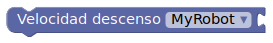
\includegraphics[width=0.4\textwidth]{img/descensoBlockly.png}
        \caption{Bloque de velocidad de descenso} \label{fig:descenso}
    \end{figure}
    \item Aterrizar: Comanda velocidad vertical al \textit{drone} hasta que alcance cierta altitud. Mantendrá esa posición hasta recibir una nueva orden.
    \begin{figure}[H]
        \centering
        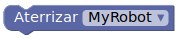
\includegraphics[width=0.3\textwidth]{img/aterrizarBlockly.png}
        \caption{Bloque de aterrizaje} \label{fig:aterrizaje}
    \end{figure}
    \item Despegar: Comanda velocidad vertical negativa al \textit{drone} hasta que alcance el suelo. 
        \begin{figure}[H]
        \centering
        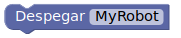
\includegraphics[width=0.3\textwidth]{img/despegarBlockly.png}
        \caption{Bloque de despegue} \label{fig:despegar}
    \end{figure}
\end{itemize}

\subsection{Modelo 3D}

Para simular el robot en el entorno de \textit{A-Frame} es necesario realizar un modelo tridimensional. Para ello se ha buscado un modelo en una librería\footnote{\url{https://sketchfab.com/}} y se ha editado en \textit{Blender} para que se ajuste a los requisitos del entorno. Las modificaciones que se han realizado al modelo son: 
\begin{itemize}
    \item Reducción de caras del \textit{drone} para que no se ralentice la carga del mundo.
    \item Rotación del modelo para que encaje con la orientación que disponía el anterior robot. Es decir, que el robot tenga su parte frontal mirando hacia el eje X positivo para que al comandarle velocidad lineal se desplace hacia delante.
    \item Modificación de la luz para adaptarla al escenario de \textit{WebSim}. 
    
    \item Elaborar una animación a las hélices para darle un aspecto más realista. Esta animación se activa vía \textit{software} cuando el drone despega del suelo. 
\end{itemize}

Además, se han incluido varios escenarios nuevos:
\begin{itemize}
    \item Uno liso para realizar pruebas y controlar el \textit{drone} sin elementos en el entorno. El drone implementado en el entorno de \textit{Websim} se puede ver en la figura \ref{fig:escenarioDrone}.
    
    \begin{figure}[H]
    \centering
    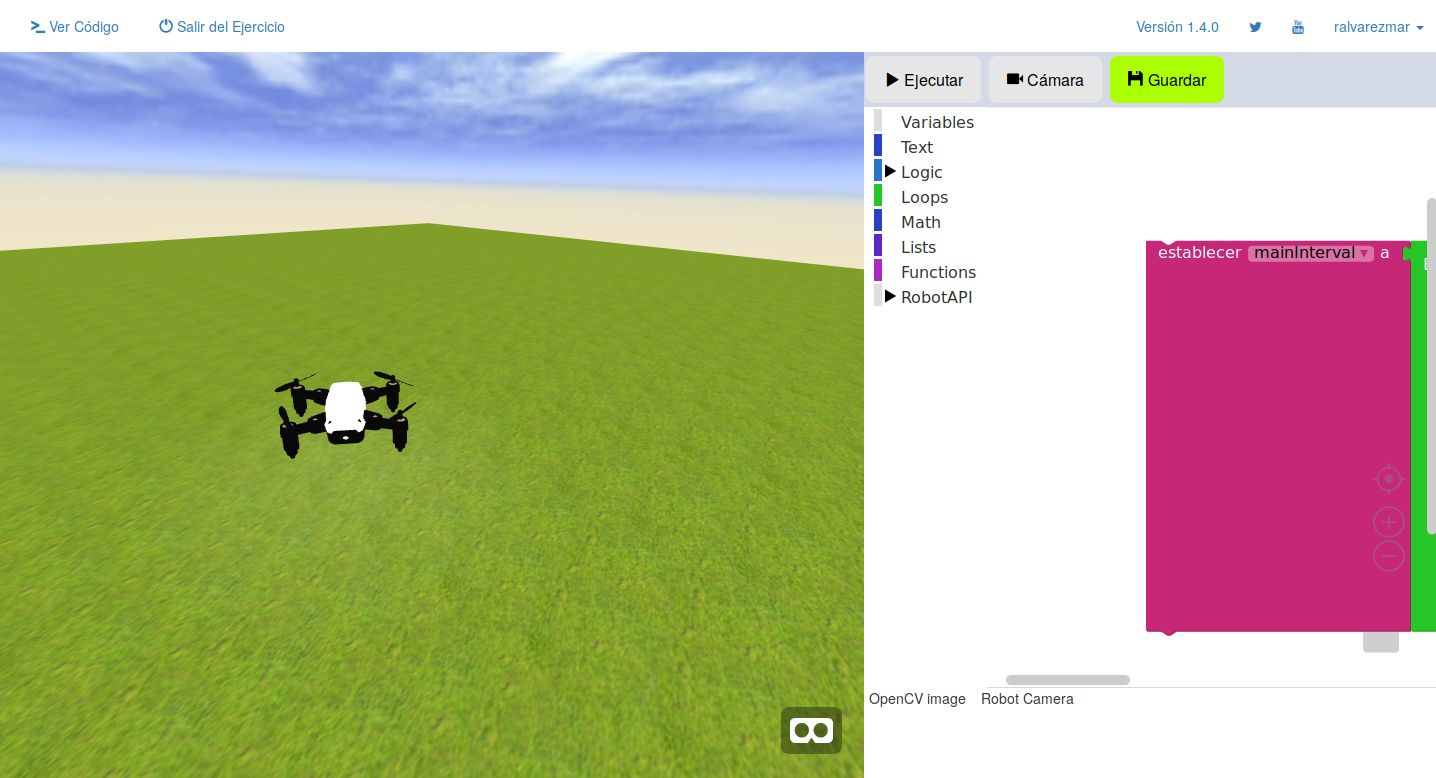
\includegraphics[scale=0.3]{img/websimDrone.png}
    \caption{Escenario de WebSim con drone integrado} \label{fig:escenarioDrone}
    \end{figure}
    
    \item Otro con un cuadrado en el suelo para facilitar el ejercicio ``cuadrado drone'' en el que hay que dibujar un cuadrado con el movimiento del drone.
    
      \begin{figure}[H]
    \centering
    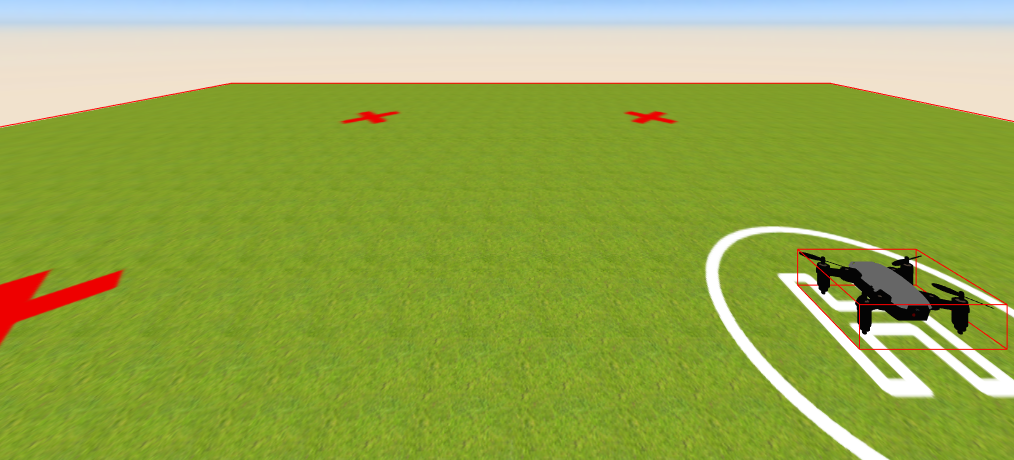
\includegraphics[scale=0.4]{img/cuadradoDrone.png}
    \caption{Escenario de WebSim para el ejercicio drone cuadrado} \label{fig:droneCuadrado}
    \end{figure}
    
    \item Un último con una pelota de color rojo en el escenario a la que se le ha dado movimiento a través de primitivas de \textit{A-Frame} para simular el ejercicio ``drone sigue-pelota''.
    \begin{figure}[H]
    \centering
    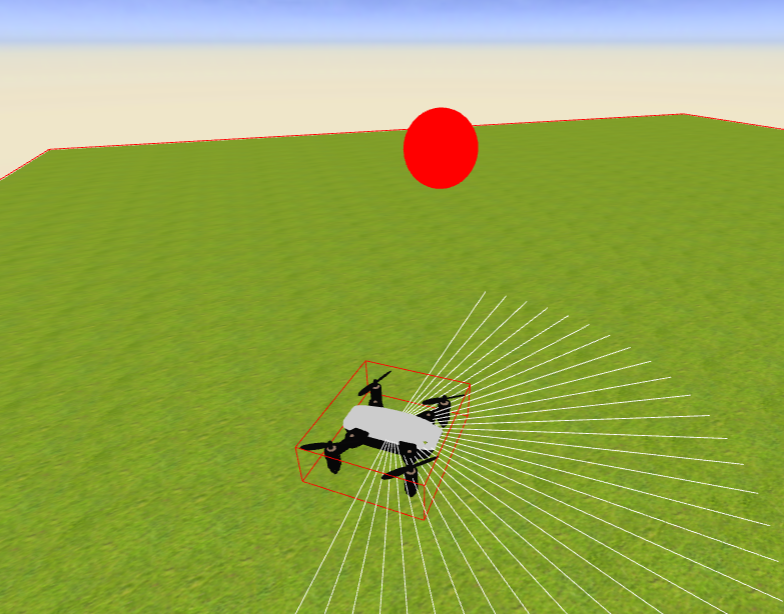
\includegraphics[scale=0.4]{img/droneBall.png}
    \caption{Escenario de WebSim para el ejercicio drone sigue-pelota} \label{fig:droneBall}
    \end{figure}
\end{itemize} 

\section{Teleoperadores}
Se han incorporado teleoperadores en \textit{WebSim} para poder controlar los robots sin necesidad de programarlos. De esta manera es posible saber el estado y valor de sus sensores de manera sencilla ayudando a los desarrolladores a buscar fallos en drivers o incorporar nuevos escenarios. 
\subsection{Archivos de configuración}

Para incorporar estos teleoperadores ha sido necesario elaborar unos ficheros de configuración y así poder cambiar el escenario y el \textit{drone} cargado por \textit{A-Frame}. \newline

\subsection{Modelos 3D}
\subsection{Aspecto gráfico}
\section{Ejercicios competitivos}
\subsection{Escenarios}
\subsection{Evaluadores automáticos}